\selectlanguage{ngerman}%
\frenchspacing%
\begin{ledgroupsized}[r]{120mm}%
\footnotesize%
\pstart%
\noindent%
\textbf{Überlieferung:}%
\pend%
\end{ledgroupsized}%
\begin{ledgroupsized}[r]{114mm}%
\footnotesize%
\pstart%
\parindent -6mm%
\makebox[6mm][l]{\textit{L}}%
Aufzeichnung:
LH XXXVII\;3 Bl.\;117.
Ein Blatt 4\textsuperscript{o};
Fragment eines \href{\Scan{LH_37_03_117wz}}{Wassezeichens}; %
Ränder beschnitten, zum Teil unregelmäßig.
Zwei ganzseitig beschriebene Seiten.
\pend%
\end{ledgroupsized}%
\vspace{5mm}%
\begin{ledgroup}%
\footnotesize%
\pstart%
\noindent%
\textbf{Datierungsgründe:}
Die Datierung der Aufzeichnung N.\;\ref{60206} beruht auf äußeren Eigenschaften des Text\-trägers %
sowie auf inhaltlichen Betrachtungen.
Siehe die ausführliche Begründung auf S.~\pageref{60206_dat}.%
\pend%
\end{ledgroup}%
\selectlanguage{latin}%
\frenchspacing%
\vspace{8mm}%
\normalsize%
\pstart%
\noindent%
\lbrack%
\href{\Scan{LH_37_03_117r}}%
{117\,r\textsuperscript{o}}%
\rbrack%
\hfill%
Pro pressione aeris%
\indexS{pressio aeris}
contra Funiculum%
\indexS{funiculus aeris}
\hfill%
\phantom{\lbrack117\,r\textsuperscript{o}\rbrack}%
\pend%
\vspace{0.5em}%
\pstart%
\noindent%
Circa naturam%
\indexS{natura aeris}
\edtext{%
aeris disceptatum est hactenus inter
Torricellium,%
\indexN{\textls{Torricelli} (Torricellius), Evangelista 1608\textendash1647} %
Pascalium,%
\indexN{\textls{Pascal} (Pascalius), Blaise 1623\textendash1662} %
Gerickium,%
\indexN{\textls{Guericke} (Gerickius, Gericke), Otto von 1602\textendash1686} %
Boylium%
\indexN{\textls{Boyle} (Boylius, Boyl), Robert 1627\textendash1691} %
et
Sinclarum%
\indexN{\textls{Sinclair} (Singlarius, Sinclarus), George gest. 1696} %
ab una;
et doctos quosdam e Societate Jesu viros,%
\indexS{vir doctus}%
\indexS{Societas Jesu}
quibus astipulantur
Franciscus Linus%
\indexN{\textls{Line} (Linus), Francis 1595\textendash1675} %
et
Thomas Albius%
\indexN{\textls{White} (Albus, Albius, Anglus), Thomas 1592/1593\textendash1676}%
\lbrack,\rbrack\
ab altera parte.%
}{%
\lemma{aeris}%
\Bfootnote{%
\bars{diu \textit{gestr.}} disceptatum est %
\textit{(1)}~inter %
\textit{(2)}~hactenus inter %
\textit{(a)}~Patres Societatis %
\textit{(b)}~Francescum, %
\textit{(c)}~Thomam Albium %
\textit{(d)}~doctos e Societate %
\textit{(e)}~Torricellium, Pascalium, Gerickium %
\textit{(aa)}~et %
\textit{(bb)}~, Boylium et Sinclarum ab una %
\textit{(aaa)}~parte, 
\textit{(bbb)}~; et doctos %
\lbrack...\rbrack\ ab altera parte.%
~\textit{L}%
}}
\edtext{%
Illi statuunt
aerem habere vim sese dilatandi
quantum possit%
\indexS{vis aeris dilatandi se}%
\indexS{vis elastica aeris}%
\lbrack,\rbrack\
\edtext{%
quam vocant Elasticam%
}{%
\lemma{quam vocant Elasticam}%
\Bfootnote{%
\textit{erg.\;L}%
}}%
}{%
\lemma{Illi \lbrack...\rbrack\ Elasticam}%
\Cfootnote{%
Siehe etwa
O.\,v.\,\textsc{Guericke},
\textit{Experimenta nova},
lib.\;III, cap.\;33
(Amsterdam 1672, S.\;116\,f.);\cite{00055}
\textsc{R.\;Boyle},
\textit{New experiments physico-mechanicall},
Nr.\;1
(Oxford 1660, S.\;20--36;\cite{00015}
\textit{BW}~I, S.\;164--170)\cite{00017}
und öfters;
\textsc{G.\;Sinclair},
\textit{Ars nova et magna gravitatis et levitatis},
lib.\;III, dialog.\;II, Nr.\;3
(Rotterdam 1669, S.\;286\,f.)\cite{00546}
und öfters.%
}}%
\lbrack;\rbrack\
\edtext{%
his contra videtur
aerem habere vim sese contrahendi%
\indexS{vis aeris contrahendi se}
instar funiculi%
\indexS{funiculus aeris}
seu chordae%
\indexS{chorda tensa}
\edlabel{LH_37_03_117_117r_saltus-1}%
tensae.%
}{%
\lemma{his \lbrack...\rbrack\ tensae}%
\Cfootnote{%
Siehe
\textsc{F.\;Line},
\textit{De corporum inseparabilitate},
cap.\;V bis cap.\;VII
(London 1661, S.\;22--29);\cite{00072}
\textsc{T.\;White}, \textit{Appendicula tentans solutionem problematis Torricelliani} %
(London 1663;\cite{00567} %
Leibnizens Handexemplar ist in der GWLB unter der Signatur Leibn.\;Marg.\;119 erhalten).
}}%
\edtext{}{%
\xxref{LH_37_03_117_117r_saltus-1}{LH_37_03_117_117r_saltus-2}%
\lemma{tensae.}%
\Bfootnote{%
\textit{(1)}~Et ideo Mercurium \textit{AB} in tubo %
\bars{\textit{BDE} \textit{erg. u. gestr.}} \textit{CB} %
\bars{intra vas \textit{DE} accurate clausum suspenso, \textit{erg.}} ad altitudinem 27 et ultra pollicum suspensum teneri putant illi a vi aeris\indexS{altitudo mercurii 27 pollicum}\indexS{pollex}\indexS{mercurius suspensus in tubo}\indexS{tubus suspensus in vase} %
\textit{(a)}~elastica in \textit{DE} contenti\indexS{vis elastica aeris} %
\textit{(b)}~in vase contenti \textls{elastica;} hi ab aeris \textit{CA} intra tubum residui \textls{funiculo}. Ponamus totum tubum \textit{CAB} fuisse Mercurio\indexS{aer residuus in tubo} %
\bars{\textit{(1)}~circiter \textit{(2)}~prope \textit{erg.}} plenum, et digito remoto\indexS{digitus remotus} %
\textit{(aa)}~partem \textit{CA} %
\textit{(bb)}~Mercuriique parte effluente in vasis \textit{DE} capacitatem, partem %
\textit{(aaa)}~va %
\textit{(bbb)}~tubi \textit{CA} remansisse aere prope vacuam; dicent illi qui Elastrum defendunt, ideo\indexS{pars tubi vacua aere} %
\textit{(2)}~Quae diversitas %
\lbrack...\rbrack\ \textit{CA} manebit aere %
\textit{(a)}~circiter vacua %
\textit{(b)}~propemodum vacua. %
\lbrack...\rbrack\ vel vas \textit{DE} %
\textit{(aa)}~accurate clausum, %
\textit{(bb)}~idque jam accuratissime %
\lbrack...\rbrack\ defendunt, statuent%
~\textit{L}%
}}
Quae diversitas maxime apparet
in explicando%
\indexS{diversitas in explicando}
\edtext{%
experimento Torricelliano.%
\indexS{experimentum Torricellianum}%
\indexS{experimentum explicandum}%
}{%
\lemma{experimento Torricelliano}%
\Cfootnote{%
Siehe \textsc{E.\;Torricelli},
Brief an M.\;Ricci vom 11.\;Juni 1644\cite{00107}
(C.\,\textsc{Dati},
\textit{Lettera a Filaleti}, %
Florenz 1663, S.\;20\,f.;\cite{00032}
\textit{TO}~III, S.\;186--188).\cite{00108}%
}}%
\pend%
\newpage%
\begin{edfigure}[0.0em][1.0em]%
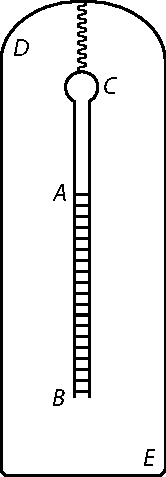
\includegraphics[width=0.18\textwidth]
{gesamttex/edit_VIII-4/images/LH_37_03_117_d1_117r.pdf}%
\edcaption[0.5em]{%
\lbrack\textit{Fig.\:1}\rbrack%
}%
\end{edfigure}%
\pstart%
Tubus \textit{CB}
clausus in \textit{C}
apertus in \textit{A}
impleatur Mercurio,%
\indexS{tubus impletus mercurio}
deinde invertatur,%
\indexS{tubus inversus}
effluet pars Mercurii,%
\indexS{mercurius effluens e tubo}
residuaque tantum manebit pars ejus \textit{AB}%
\indexS{pars mercurii residua}
altitudinis plus minus 27 pollicum,%
\indexS{altitudo mercurii 27 pollicum}%
\indexS{pollex}
et pars tubi \textit{CA} manebit aere propemodum vacua.%
\indexS{pars tubi vacua}
Tubus hoc modo inversus%
\indexS{tubus inversus}
cum Mercurio in eo suspenso,%
\indexS{mercurius suspensus in tubo}
suspendatur intra alium tubum%
\indexS{tubus suspensus in tubo}
vel vas \textit{DE},
idque jam accuratissime claudatur.%
\indexS{tubus clausus accurate}
Qui vim Elasticam defendunt,%
\indexS{vis elastica aeris}
statuent%
\edlabel{LH_37_03_117_117r_saltus-2}
aerem \textit{DE}
elastro suo se dilatare conantem%
\indexS{elastrum aeris}%
\indexS{aer conans dilatare se}
conari Mercurium \textit{AB} intra%
\indexS{mercurius suspensus in tubo}
\edtext{%
tubum supra \textit{A} pellere,%
}{%
\lemma{tubum}%
\Bfootnote{%
\textit{(1)}~\textit{CA} %
\textit{(2)}~supra \textit{A} pellere,%
~\textit{L}%
}}
idque
\edtext{%
facturum esse%
}{%
\lemma{facturum}%
\Bfootnote{%
\textit{(1)}~esset %
\textit{(2)}~esse%
~\textit{L}%
}}
nisi
\edtext{%
pondus 27 pollicum Mercurii%
\indexS{pondus mercurii 27 pollicum}%
\indexS{pollex}%
}{%
\lemma{pondus}%
\Bfootnote{%
\textit{(1)}~Mercurii %
\textit{(2)}~27 pollicum Mercurii%
~\textit{L}%
}}
cum ejus elastro esset in aequilibrio.%
\indexS{elastrum aeris}%
\indexS{aequilibrium mercurii cum elastro aeris}
Contra%
\lbrack,\rbrack\
\edtext{%
autores funiculi%
\indexS{autores funiculi}%
\indexS{funiculus aeris}
dicent Mercurium
\edtext{%
\textit{AB}%
}{%
\lemma{\textit{AB}}%
\Bfootnote{%
\textit{erg.\;L}%
}}
effluere conantem%
\indexS{mercurius effluens e tubo}%
\lbrack,\rbrack\
secum extendere aerem%
\indexS{mercurius extendens aerem residuum}
\edtext{%
quantulumcunque%
\indexS{aer quantuluscunque}
intra tubum residuum%
\indexS{aer residuus in tubo}%
}{%
\lemma{quantulumcunque}%
\Bfootnote{%
\textit{(1)}~inclusum %
\textit{(2)}~intra tubum residuum%
~\textit{L}%
}}
\textit{CA},
et omnino effluxurum esse%
\indexS{mercurius effluens e tubo}
nisi a funiculo aeris,%
\indexS{funiculus aeris}
velut pondus a chorda tensa,%
\indexS{chorda tensa}%
\indexS{pondus retentum a chorda tensa}
retineretur.%
\indexS{mercurius retentus a funiculo aeris}%
}{%
\lemma{autores \lbrack...\rbrack\ retineretur}%
\Cfootnote{%
Leibnizens Darstellung deckt sich nur begrenzt mit Lines\indexN{\textls{Line} (Linus), Francis 1595\textendash1675} Erklärung von Torricellis\indexN{\textls{Torricelli} (Torricellius), Evangelista 1608\textendash1647} Experiment; vgl. \textit{De corporum inseparabilitate}, cap.\;XI (S.\;49--51).\cite{00072}
Line betont vielmehr, dass das \textit{vinculum}, das die Quecksilbersäule in der Rohr vom Sinken abhält, aus verdünntem Quecksilber besteht, nicht aus restlicher Luft; vgl. ebd., cap.\;X (S.\;37--45).\cite{00072}
Leibnizens Darstellung zeigt auch mit Whites\indexN{\textls{White} (Albus, Albius, Anglus), Thomas 1592/1593\textendash1676} Erklärung begrenzt Verwandschaft; vgl. \textit{Appendicula}, prop.\;II u.\;III (S.\;8--10).\cite{00567}%
}}
Verum in Hypothesi funiculi%
\indexS{hypothesis funiculi aeris}%
\indexS{funiculus aeris}
reddenda est ratio determinatae altitudinis Mercurii,%
\indexS{altitudo mercurii determinata}%
\indexS{ratio altitudinis mercurii reddenda}%
\indexS{mercurius suspensus in tubo}
quae in Hypothesi Elastri%
\indexS{hypothesis elastri aeris}%
\indexS{elastrum aeris}
est manifesta.%
\indexS{ratio manifesta}
Imo in Hypothesi funiculi%
\indexS{hypothesis funiculi aeris}%
\indexS{funiculus aeris}
determinata hujusmodi altitudo%
\indexS{altitudo mercurii determinata}
servari non potest,
nam aeris%
\indexS{aer latens in mercurio}\indexS{aer intra tubum et mercurium}
\edtext{%
in Mercurio vel intra%
}{%
\lemma{in}%
\Bfootnote{%
\textit{(1)}~Tubo vel intra %
\textit{(2)}~Mercurio vel intra%
~\textit{L}%
}}
tubum et Mercurium latentis
pro varia tubi superficie concava%
\indexS{tubus impletus mercurio}
(quae capacitati minime proportionalis est)
varia esse potest quantitas;
et ita effici poterit
ut aer tantillus%
\indexS{aer tantillus}
intra \textit{CA} residuus,%
\indexS{aer residuus in tubo}
duplo fiat dilatatior%
\indexS{aer dilatatus}
\edtext{%
in uno casu quam in alio,%
}{%
\lemma{in uno %
\lbrack...\rbrack\ in alio}%
\Bfootnote{%
\textit{erg.\;L}%
}}
unde duplo pondere dilatante,%
\indexS{pondus mercurii dilatans aerem}
\edtext{%
seu duplicata%
}{%
\lemma{seu}%
\Bfootnote{%
\textit{(1)}~duplici %
\textit{(2)}~duplicata%
~\textit{L}%
}}
Mercurii altitudine opus esset.%
\indexS{altitudo mercurii suspensi in tubo}%
\indexS{mercurius suspensus in tubo}
Accedit
quod diversi liquores%
\indexS{liquor}
servant altitudinem ponderibus reciproce proportionalem,%
\indexS{altitudo liquoris reciproce proportionalis ponderi}
cum tamen ratione aeris%
\indexS{ratio aeris contenti in tubo}%
\indexS{aer contentus in tubo}
\edtext{%
contenti in tubo variare deberent.%
}{%
\lemma{contenti}%
\Bfootnote{%
\bars{in tubo \textit{erg.}} variare %
\textit{(1)}~debeant %
\textit{(2)}~deberent%
~\textit{L}%
}}
Itaque
licet
aerem aliquem in tubo superesse%
\indexS{aer residuus in tubo}
non sit negandum,
tantillam tamen
\edtext{%
ejus quantitatem esse oportet,
ut%
}{%
\lemma{ejus}%
\Bfootnote{%
\textit{(1)}~quantitas est, ut oportet %
\textit{(2)}~quantitatem esse oportet, ut%
~\textit{L}%
}}
majoris minorisque ejus dilatationis%
\indexS{dilatatio aeris residui in tubo}
rationem haberi non sit opus,
unde funiculus%
\indexS{funiculus aeris}
locum habere non
\edtext{%
potest,
quod%
}{%
\lemma{potest,}%
\Bfootnote{%
\textit{(1)}~idque %
\textit{(2)}~quod%
~\textit{L}%
}}
imposterum habendum erit pro demonstrato
et ex ipsa societate%
\indexS{Societas Jesu}
\edtext{%
\edlabel{LH_37_03_117_117r_Dechales-1}%
agnitum est a Chalesio%
\indexN{\textls{Dechales} (Chalesius), Claude François Milliet 1621\textendash1678}%
\edlabel{LH_37_03_117_117r_Dechales-2}%
}{%
\lemma{agnitum \lbrack...\rbrack\ Chalesio}%
\Cfootnote{%
Wohl Anspielung auf
\textsc{C.\;Dechales}, \textit{Cursus seu mundus mathematicus},
tract.\;VII, lib.\;I, digr.\;V--VII (Lyon 1674, Bd.\;I, S.\;436a--448b):\cite{00124}
Torricellis\indexN{\textls{Torricelli} (Torricellius), Evangelista 1608\textendash1647} Experiment wird dort lediglich unter Berücksichtigung des Luftgewichts erklärt, während Lines\indexN{\textls{Line} (Linus), Francis 1595\textendash1675} alternative Erklärung unerwähnt bleibt.
Aus dem nachgewiesenen Abschnitt aus Deschales' \textit{Cursus}\cite{00124} hat Leibniz Exzerpte verfasst; siehe N.\;\ref{41182-1} im vorliegenden Band.%
}}
viro maxime ingenuo et judicioso.%
\indexS{vir ingenuus}%
\indexS{vir judiciosus}
\lbrack%
\href{\Scan{LH_37_03_117v}}%
{117\,v\textsuperscript{o}}%
\rbrack\ %
\edlabel{LH_37_03_117_117v_PaderbornJS-1}%
Addatur
\edtext{%
Epistola%
\indexS{epistola}
quam ad Jesuitam%
\indexN{Jesuita mathematicus Paderbornensis}%
\indexS{mathematicus}
\edtext{%
Mathematicum Padebornensem\indexO{Paderborn}%
}{%
\lemma{Mathematicum}%
\Bfootnote{%
\textit{(1)}~Osnabrugensem %
\textit{(2)}~Padebornensem%
~\textit{L}%
}}
de hoc argumento scripsi anno 1681.%
\indexS{argumentum}%
\edlabel{LH_37_03_117_117v_PaderbornJS-2}%
}{%
\lemma{Epistola \bracks{...} 1681}%
\Cfootnote{%
Nicht nachgewiesen.}}
\pend%
\pstart%
Interea
ut dicam
quod res
\edtext{%
est,
non videtur aer per se ac sua natura esse Elasticus,%
\indexS{aer non elasticus per se ac sua natura}%
\indexS{natura aeris}
nec%
}{%
\lemma{est,}%
\Bfootnote{%
\textit{(1)}~non puto in aere proprie vim E\indexS{vis elastica aeris} %
\textit{(2)}~non videtur %
\lbrack...\rbrack\ esse Elasticus, %
\textit{(a)}~nec %
\textit{(b)}~nec%
~\textit{L}%
}}
magis dicendum est
aerem habere per se vim sese dilatandi,%
\indexS{vis aeris dilatandi se}%
\indexS{aer non habens per se vim dilatandi}
quam contrahendi.%
\indexS{vis aeris contrahendi se}%
\indexS{aer non habens per se vim contrahendi}
Licet enim fingamus
aerem esse instar lanae%
\indexS{aer instar lanae}%
\indexS{lana}
constareque ex partibus ramosis rigidis%
\indexS{aer constans e partibus ramosis rigidis}%
\indexS{partes aeris ramosae rigidae}
ac si premantur se restituentibus,
nova quaestio erit,
undenam hae partes suum habeant Elastrum.%
\indexS{elastrum partium aeris}
\edlabel{LH_37_03_117_117r_explmechelstr-1}%
Dicendum est ergo%
\lbrack,\rbrack\
\edtext{%
quod alibi fusius explicui,%
}{%
\lemma{alibi}%
\Cfootnote{%
Möglicherweise Anspielung auf den Entwurf \textit{Explicatio mechanica elastri}, \textit{LSB} VIII,\;3 N.\;14\textsubscript{3}\cite{01437} \bracks{Ende Januar -- März\:/\:April 1683}.%
}}
fluidum aetherium cuncta pervadens%
\indexS{fluidum aetherium pervadens cuncta}
celerrimo suo motu%
\indexS{motus fluidi aetherei}
partes aeris dispergere et dissipare conari%
\lbrack,\rbrack\
prorsus ut aqua calore ebullit%
\indexS{aqua ebulliens calore}
\edtext{%
et pulvis%
\indexS{pulvis disgregatus a vento}
aut plumae%
\indexS{plumae disgregatae a vento}%
}{%
\lemma{et}%
\Bfootnote{%
\textit{(1)}~fumae %
\textit{(2)}~pulvis aut plumae%
~\textit{L}%
}}
vento perflante%
\indexS{ventus perflans}
disgregantur.%
\edlabel{LH_37_03_117_117r_explmechelstr-2}
Sed cum idem motus%
\indexS{motus fluidi aetherei}
corpora
quae dispergere non potest
\edtext{%
ita colligat,%
}{%
\lemma{ita}%
\Bfootnote{%
\textit{(1)}~componat %
\textit{(2)}~colligat%
~\textit{L}%
}}
ut quam minimum ab illis turbetur,
et ita versus centrum globi nostri detrudat,%
\indexS{corpora detrusa versus centrum terrae}%
\indexS{centrum globi nostri}
luctantur inter%
\indexS{lucta inter gravitatem et elastrum aeris}
\edtext{%
se gravitas%
\indexS{gravitas aeris}
et Elastrum,%
\indexS{elastrum aeris}
et elastrum unius partis
cum elastro alterius partis,
unde partes aeris
ad eundem consistentiae gradum%
\indexS{gradus consistentiae aeris}%
\indexS{consistentia aeris}
sese qua possunt componunt,
nisi quod%
}{%
\lemma{se}%
\Bfootnote{%
\textit{(1)}~conatus gravitat %
\textit{(2)}~gravitas et Elastrum, et %
\textit{(a)}~quand %
\textit{(b)}~licet %
\textit{(aa)}~servata %
\textit{(bb)}~servatur uniformitas %
\textit{(c)}~elastrum unius %
\lbrack...\rbrack\ ad eundem %
\textit{(aa)}~tensionis sive ela %
\textit{(bb)}~consistentiae gradum %
\lbrack...\rbrack\ nisi quod%
~\textit{L}%
}}
ob gravitatem%
\indexS{gravitas aeris}
magis pressae sunt inferiores%
\indexS{pars aeris inferior}
quam superiores.%
\indexS{pars aeris superior}
\pend%
\pstart%
Caeterum adjicere hic placet
\edlabel{LH_37_03_117_117v_morland-1}%
responsionem ad%
\indexS{responsio ad objectionem}
\edtext{%
objectionem mire%
}{%
\lemma{objectionem}%
\Bfootnote{%
\textit{(1)}~per %
\textit{(2)}~mire%
~\textit{L}%
}}
elegantem ipsius
\edtext{%
Magnae Britanniae Regis%
\indexN{\textls{England: Karl II.}, König 1660\textendash1685}%
}{%
\lemma{Magnae Britanniae Regis}%
\Cfootnote{%
Der von 1660 bis 1685 regierende König von England\indexO{England} Karl II.%
}}
pro funiculo factam%
\indexS{responsio pro funicolo}
et a Samuele
\edtext{%
Morelando%
\indexN{\textls{Morland} (Moreland), Samuel 1625\textendash1695}%
}{%
\lemma{Morelando}%
\Cfootnote{%
Nicht nachgewiesen.
Siehe aber Leibnizens Brief an N.\;Grew vom 9./19.\;Marz 1680:
\textit{Vidi schedam quandam Domini Morlandi,\indexN{\textls{Morland} (Moreland), Samuel 1625\textendash1695} quibus refutare conatur aequilibrium cylindri aerei, sed ex observatione ejus, quanquam ea non inelegans sit, nescio an quod ille voluit concludatur.}
(\textit{LSB} III,\;3 N.\;32, S.\;88.14--16).\cite{02600}%
}}
relatam.%
\edlabel{LH_37_03_117_117v_morland-2}
Nempe
\edtext{%
tubus%
\indexS{tubus inversus}%
\indexS{tubus suspensus e libra}
\edtext{%
inversus%
}{%
\lemma{inversus}%
\Bfootnote{%
\textit{erg.\;L}%
}}
\textit{CAB},%
}{%
\lemma{tubus inversus \textit{CAB}}%
\Cfootnote{%
Vgl. das Diagramm \bracks{\textit{Fig.\:2}}.%
}}
\edtext{%
clausus in \textit{C},
apertus in \textit{B},%
}{%
\lemma{clausus in \textit{C},
apertus in \textit{B},}%
\Bfootnote{%
\textit{erg.\;L}%
}}
cujus pars superior \textit{AC} vacua%
\indexS{pars tubi vacua aere}
communi aere,%
\indexS{aer communis}
pars autem
\edtext{%
\textit{AB}
27 circiter pollicum%
\indexS{pollex}
plena est Mercurio pensili;%
\indexS{mercurius pensilis 27 pollicum}
suspendatur%
}{%
\lemma{\textit{AB}}%
\Bfootnote{%
\bars{27 circiter pollicum \textit{erg.}} plena est %
\textit{(1)}~Mercurius 27 circiter po %
\textit{(2)}~Mercurio %
\textit{(a)}~suspenso %
\textit{(b)}~pensili; %
\textit{(aa)}~totus autem tubus %
\textit{(bb)}~suspendatur%
~\textit{L}%
}}
ex librae \textit{DEF} brachio \textit{ED} in \textit{D},%
\indexS{brachium librae}%
\indexS{libra}%
\indexS{tubus suspensus e libra}
et ab altero brachio \textit{EF} in \textit{F}
suspendatur pondus \textit{G},%
\indexS{pondus suspensum e libra}
\edtext{%
reperietur non haberi aequilibrium,%
\indexS{aequilibrium brachiorum librae}
nisi pondus aequivaleat%
}{%
\lemma{reperietur}%
\Bfootnote{%
\textit{(1)}~pondus ut in %
\textit{(2)}~non haberi %
\lbrack...\rbrack\ pondus aequivaleat%
~\textit{L}%
}}
non tantum tubo vitreo,%
\indexS{tubus vitreus includens hydrargyrum}
sed et Hydrargyro incluso.%
\indexS{hydrargyrum inclusum in tubo}
Unde colligi videtur,
Mercurium non%
\indexS{mercurius sustentus ab aere}
\edtext{%
sustineri ab aere%
}{%
\lemma{sustineri}%
\Bfootnote{%
\textit{(1)}~aere %
\textit{(2)}~ab aere%
~\textit{L}%
}}
ambiente%
\indexS{aer ambiens}%
\lbrack,\rbrack\
alioqui cum tubo non ponderaret,
sed potius Mercurium ope%
\indexS{mercurius pendens ope funiculi aerei}
\edtext{%
funiculi aerei ex tubo pendere.%
}{%
\lemma{funiculi}%
\Bfootnote{%
\textit{(1)}~ex tubo pend %
\textit{(2)}~aerei ex tubo pendere%
~\textit{L}%
}}
Responderi potest %
primum per instantiam,%
\indexS{responsio per instantiam}%
\indexS{instantia}
ubi negari non potest Mercurium%
\indexS{mercurius sustentus a liquido ambiente}
\edtext{%
ab ambiente liquido%
\indexS{liquidum ambiens}%
}{%
\lemma{ab}%
\Bfootnote{%
\textit{(1)}~aere %
\textit{(2)}~ambiente liquido%
~\textit{L}%
}}
sustentari,
nempe si
\edtext{%
experimentum Torricellianum%
\indexS{experimentum Torricellianum}
fiat%
}{%
\lemma{experimentum}%
\Bfootnote{%
\textit{(1)}~fiat %
\textit{(2)}~Torricellianum fiat%
~\textit{L}%
}}
in fundo maris,%
\indexS{fundus maris}%
\indexS{mare}
ubi longe altius extabit Mercurius,%
\indexS{altitudo mercurii in fundo maris}%
\indexS{mercurius extans in tubo}
\edtext{%
ad 50 et%
}{%
\lemma{ad}%
\Bfootnote{%
\textit{(1)}~40 et %
\textit{(2)}~50 et%
~\textit{L}%
}}
amplius pollices%
\indexS{pollex}
pro maris profunditate,%
\indexS{profunditas maris}%
\indexS{mare}
et nihilo minus
\edtext{%
pondus totius Mercurii,%
\indexS{pondus mercurii sustenti a cylindro aquae}
etiam quem aquae cylinder sustinet%
\indexS{mercurius sustentus a cylindro aquae}%
\indexS{cylinder aquae}%
\lbrack,\rbrack\
a librante in fundo maris%
\indexS{fundus maris}%
}{%
\lemma{pondus}%
\Bfootnote{%
\textit{(1)}~non tubi tantum, sed et %
\textit{(2)}~totius Mercurii, %
\lbrack...\rbrack\ cylinder sustinet %
\textit{(a)}~in libra %
\textit{(b)}~in maris fundo %
\textit{(c)}~a librante in fundo maris%
~\textit{L}%
}}
certissime sentietur,
nec dubitem pignore%
\indexS{pignus}
hac de re certare.
Deinde ad argumentum ipsum respondendum
\edtext{%
est fluidum ambiens%
\indexS{fluidum ambiens}%
}{%
\lemma{est}%
\Bfootnote{%
\textit{(1)}~aere %
\textit{(2)}~fluidum ambiens%
~\textit{L}%
}}
sustinere pondus Mercurii%
\indexS{pondus mercurii sustentum a fluido ambiente}%
\indexS{mercurius sustentus a fluido ambiente}
non omnino
(neque enim impedit,
quin una cum tubo
\edtext{%
descendat
cum tubus librae appenditur)%
\indexS{tubus appensus librae}%
\indexS{libra}%
}{%
\lemma{descendat}%
\Bfootnote{%
\textit{(1)}~ut fit in libra, %
\textit{(2)}~cum tubus librae appenditur)%
~\textit{L}%
}}
sed hactenus
\edtext{%
tantum,
ne%
}{%
\lemma{tantum,}%
\Bfootnote{%
\textit{(1)}~ut %
\textit{(2)}~ne%
~\textit{L}%
}}
sine tubo descendat,
\edtext{%
seu ne a%
}{%
\lemma{seu}%
\Bfootnote{%
\bars{ne \textit{erg.}} a%
~\textit{L}%
}}
tubo separetur.
Idemque ad duo
\edtext{%
Marmora polita sibi adhaerentia,%
\indexS{marmora polita adhaerentia}%
}{%
\lemma{Marmora}%
\Bfootnote{%
\textit{(1)}~sibi adhae %
\textit{(2)}~polita sibi adhaerentia,%
~\textit{L}%
}}
aliosque casus applicari potest.
\pend%
\newpage%
\begin{edfigure}[2.0em][0.0em]%
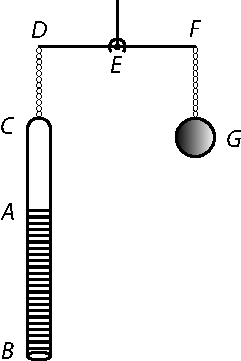
\includegraphics[width=0.26\textwidth]
{gesamttex/edit_VIII-4/images/LH_37_03_117_d2_117v.pdf}%
\edcaption[0.25em]{%
\lbrack\textit{Fig.\:2}\rbrack%
}%
\end{edfigure}%
\vspace*{4.5em}%
\pstart%
\noindent%
\centering%
*     *     *
\pend%
\vspace{4.5em}%
\selectlanguage{german}%
\frenchspacing%
\footnotesize%
\pstart%
\noindent%
\textls{Ausführliche Datierungsgründe:}%
\pagelabel{60206_dat}
Die undatierte Aufzeichnung N.\;\ref{60206} \textit{Pro pressione aeris, contra funiculum} knüpft gleich zu Beginn an die Auseinandersetzung an, die in den frühen 1660er Jahren Verfechter des elastischen Verhaltens der Luft wie etwa Robert Boyle\indexN{\textls{Boyle} (Boylius, Boyl), Robert 1627\textendash1691} und Anhänger der "Funiculus"-Lehre wie Francis Line\indexN{\textls{Line} (Linus), Francis 1595\textendash1675} oder Thomas White\indexN{\textls{White} (Albus, Albius, Anglus), Thomas 1592/1593\textendash1676} entfachteten. %
Leibniz nimmt hierbei, wie der Titel selbst zeigt und wie bereits in der inhaltlich verwandten Aufzeichnung N.\ref{60261} der Fall war, gegen die "Funiculus"-Lehre Stellung.
Die für die Aufzeichnung N.\;\ref{60206} vorgeschlagene Datierung ergibt sich aus folgenden Beobachtungen:
\pend%
\pstart%
(1)
Im Träger von N.\;\ref{60206} ist das Fragment eines Harzer \href{\Scan{LH_37_03_117wz}}{Wassezeichens} (Wilder Mann mit Glocke und Jahresangabe 1678) anzutreffen, %
das im Leibniz-Nachlass nach heutigem Wissensstand %
für die Zeitspanne 1679 bis 1685 belegt ist;
dieses Papier wird im Nachlass ab 1686 durch ähnliches (mit gleichem Wasserzeichen, aber Jahresangabe 1685) ersetzt.
Die Eigenschaften des Fragments im Träger von N.\;\ref{60206} zeigen, dass es sich hierbei um die ältere Papiersorte handelt. %
\pend%
\pstart%
(2)
In N.\;\ref{60206} (\refpassage{LH_37_03_117_117v_PaderbornJS-1}{LH_37_03_117_117v_PaderbornJS-2}) verweist Leibniz auf einen Brief, den er im Jahr 1681 an einen nicht ermittelten jesuitischen Mathematiker aus Paderborn\indexN{Jesuita mathematicus Paderbornensis}\indexO{Paderborn} geschrieben haben soll.
Folglich kann die Aufzeichnung N.\;\ref{60206} frühestens im Jahr 1682 abgefasst worden sein.
Da Leibniz bei seiner Andeutung, statt eine Wendung zu benutzen wie \textit{anno priore} oder \textit{superiore}, die Jahreszahl angibt, erweist sich als wahrscheinlich, dass N.\;\ref{60206} nicht vor 1683 verfasst wurde.
\pend%
\pstart%
(3)
Ausschlaggebend für die Bestimmung des Terminus post quem der Datierung dürfte vorwiegend der Umstand sein, dass in N.\;\ref{60206} (\refpassage{LH_37_03_117_117r_Dechales-1}{LH_37_03_117_117r_Dechales-2}) auf \textsc{C.\;Dechales}, \textit{Cursus seu mundus mathematicus},
tract.\;VII, lib.\;I, digr.\;V--VII (Lyon 1674, Bd.\;I, S.\;436a--448b)\cite{00124} angespielt wird.
Mit Dechales'\indexN{\textls{Dechales} (Chalesius), Claude François Milliet 1621\textendash1678} \textit{Cursus seu mundus mathematicus}\cite{00124} hat sich Leibniz wohl zwischen dem Winter 1682/1683 und der ersten Hälfte 1685 befasst, wie die im vorliegenden Band veröffentlichten Auszüge mit Bemerkungen N.\;\ref{41182-1} und N.\;\ref{41182-2} zeigen (siehe dort die ausführlichen Datierungsgründe, S.\;\pageref{41182_dat}).
Hieraus ist zu schließen, dass die Aufzeichnung N.\;\ref{60206} wahrscheinlich nicht vor dem Winter 1682/1683 angefertigt wurde, vermutlich nicht vor Anfang 1683.
Falls die Vermutung ferner zutrifft, dass N.\;\ref{60206} (\refpassage{LH_37_03_117_117r_explmechelstr-1}{LH_37_03_117_117r_explmechelstr-2}) auf den zwischen Ende Januar und März\:/\:April 1683 entstandenen Entwurf \textit{Explicatio mechanica elastri} (\textit{LSB} VIII,\;3 N.\;14\textsubscript{3})\cite{01437} anspielt, dann würde dies den vorgeschlagenen Terminus post quem weiterhin bestätigen.
\pend%
\pstart%
(4)
Zur Bestimmung des Terminus ante quem trägt die Feststellung bei, dass die Aufzeichnung N.\;\ref{60206} (\refpassage{LH_37_03_117_117v_morland-1}{LH_37_03_117_117v_morland-2}) aller Wahrscheinlichkeit nach auf eine nicht ermittelte \textit{scheda} von Samuel Morland\indexN{\textls{Morland} (Moreland), Samuel 1625\textendash1695} verweist, deren Inhalt Leibniz in seinem Brief an Nehemiah Grew\indexN{\textls{Grew}, Nehemiah 1641\textendash1712} vom 9./19.\;Marz 1680 kurz zusammenfasst (\textit{LSB} III,\;3 N.\;32, S.\;88.14--16; siehe die Erläuterung zu N.\;\ref{60206}, \refpassage{LH_37_03_117_117v_morland-1}{LH_37_03_117_117v_morland-2}).\cite{02600}
Demnach ist anzunehmen, dass der König von England,\indexO{England} über den Morland\indexN{\textls{Morland} (Moreland), Samuel 1625\textendash1695} in der besagten \textit{scheda} berichtet haben soll und auf den sich Leibniz als amtierenden Monarch bezieht, der am 6.\;Februar 1685 verstorbene Karl~II. sein muss.\indexN{\textls{England: Karl II.}, König 1660\textendash1685}
Von dessen Tod wusste Leibniz bereits einen Monat später, wie sein Brief vom 4./14.\;März 1685 an Landgraf Ernst von Hessen-Rheinfels\indexN{\textls{Hessen-Rheinfels: Ernst}, Landgraf 1649\textendash1693} nachweist (\textit{LSB} I,\;4 N.\;308, S.\;349.4\,f.).\cite{02601}
Dies ist Grund für die Annahme, dass N.\;\ref{60206} spätestens im Februar 1685 angefertigt wurde, wohl aber schon etwas früher.
\pend%
\pstart%
Aus diesen Betrachtungen ergibt sich als wahrscheinliche Gesamtdatierung der vorliegenden Aufzeichnung N.\;\ref{60206} \textit{Pro pressione aeris, contra funiculum} der Zeitraum 1683--1684.
Eine frühere (ab 1682) oder eine spätere (bis 1685) Entstehung sind nicht auszuschließen, aber unwahrscheinlich.
\pend%
\selectlanguage{latin}%
\frenchspacing%
\newpage%
